\section{Classifier}

\subsection{Architecture}
We explored different architectures for the convolutional neural network (CNN) for split error detection. In table \ref{tab:architecture} we compare traditional CNN architectures versus residual networks~\cite{resnet}. The traditional architecture with dropout regularization generalized better than residual networks on unseen testing data.

\begin{table}[h]
\caption{Traditional CNN Architecture versus Residual Network Architecture \cite{resnet}. All configurations are compared using the same parameters. Our final choice (indicated by *) trains relatively fast and performs better.}%While the training of our classifier is more expensive, testing accuracy is superior. }

\small{
\begin{tabular}{@{}ll|l@{}}
	\toprule
     ~ & \textbf{Traditional Network} & \textbf{Residual Network}  \\ \midrule	
\begin{tabular}{@{}r|@{}}
Conv. Layers \\
Dropout Reg. \\
Cost [m] \\
Test. Acc. \\
Prec./Recall \\
F1 Score\\
~
\end{tabular} & 
\begin{tabular}{@{}c|c@{}}
 2 & 4 \\
 y & y \\
 27.5 & 383 \\
 0.925 & 0.94 \\
 0.93/0.93 &
 0.94/0.94 \\
 0.93 & 0.94 \\
 ~&*
\end{tabular}
& 
\begin{tabular}{@{}c|c@{}}
 5 & 13 \\
 y & n \\
5080 & 1094 \\
 0.93 & 0.90 \\
 0.7/0.53 &
 0.74/0.66 \\
 0.39 & 0.64\\
 ~&~

\end{tabular}

\end{tabular}
\hspace{2mm}
\hrule
}
\label{tab:architecture}
\end{table}




\subsection{Training Parameters}

We performed a limited brute force parameter search to tune the split error classifier (Tab. \ref{tab:parametersearch}). This resulted in 3240 different CNN configurations which were evaluated on 10\% of our training data. Learning rate and momentum ranges are defined linearly across 2000 epochs.

\begin{table}[h]
\caption{Brute force parameter search for the split error classifier. The final parameters are highlighted.}%While the training of our classifier is more expensive, testing accuracy is superior. }

\small{
\begin{tabular}{@{}ll}
	\toprule
     \textbf{Parameter} & \textbf{Search Space}  \\ \midrule	
\begin{tabular}{@{}l@{}}
Filter size: \\
No. Filters 1: \\
No. Filters 2-4: \\
Dense units:\\
Learning rate: \\
Momentum: \\
Mini-Batchsize: 
\end{tabular} & 
\begin{tabular}{@{}l@{}}
\textbf{3x3}, 5x5, 9x9, 13x13\\
32, 48, \textbf{64} \\
32, \textbf{48}, 64 \\
256, \textbf{512} \\
0.00001, 0.0001, 0.001, 0.01, \textbf{0.03-0.00001} \\
0.9, 0.95, \textbf{0.9-0.999} \\
10, 100, \textbf{128}
\end{tabular}

\end{tabular}
\hspace{2mm}
\hrule
}
\label{tab:parametersearch}
\end{table}

\subsection{Automatic Method Threshold $p_t$}
For automatic selection, we observed a threshold $p_t=0.95$ as stable when evaluating on previously unseen testing data (Mouse S1 AC3 Open Connectome Project dataset). This means, that automatic selection stops once all borders with $p_t\geq0.95$ were proofread. Fig. \ref{fig:pt} shows split error classification on three randomly selected subvolumes ($700\times700\times2$ voxels) of AC3. In all cases, the threshold $p_t=0.95$ reduces VI.

\begin{figure}[t]
\centering
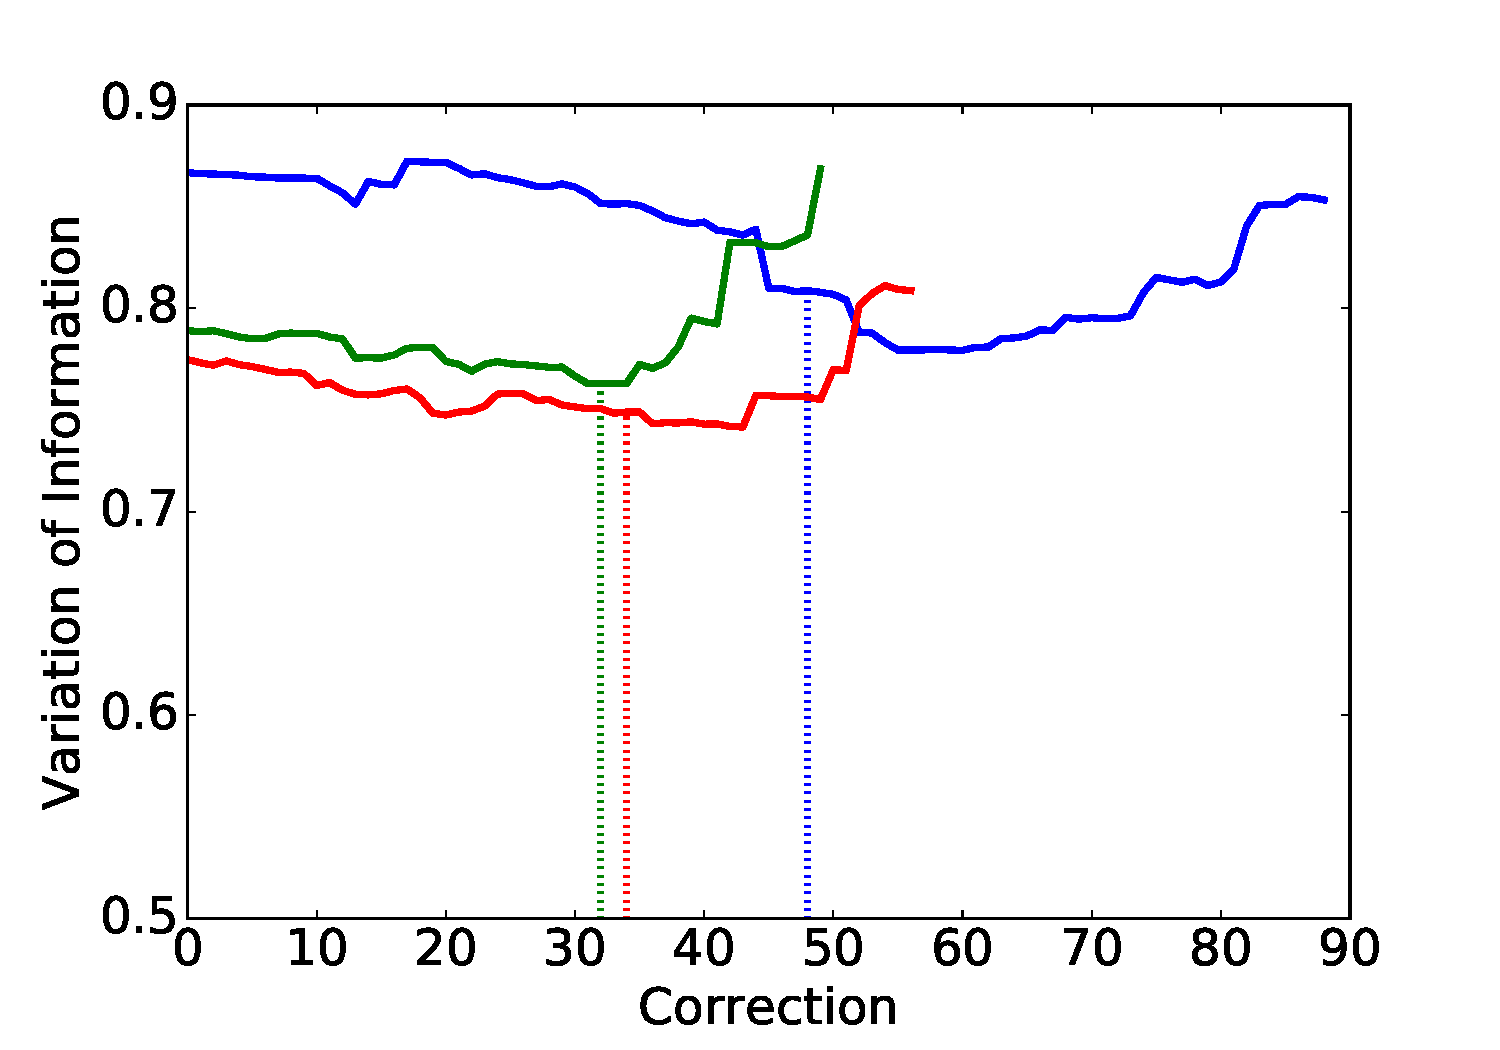
\includegraphics[width=\linewidth]{gfx/ptplot.pdf}
\caption{Observations of probability thresholds $p_t$ during automatic selection on three different subvolumes of previously unseen testing data. The dashed lines show when $p_t=0.95$ is reached.}
\label{fig:cylboxplot}
\end{figure}

\subsection{Limitations}
Guided proofreading works on 2D image sections. This enables error correction without a computationally expensive alignment process. However, the output requires an additional (block-)merging step prior to 3D  analysis.
